\documentclass{standalone}
\usepackage{tikz}
\usetikzlibrary{calc}
\usetikzlibrary{positioning}
\begin{document}
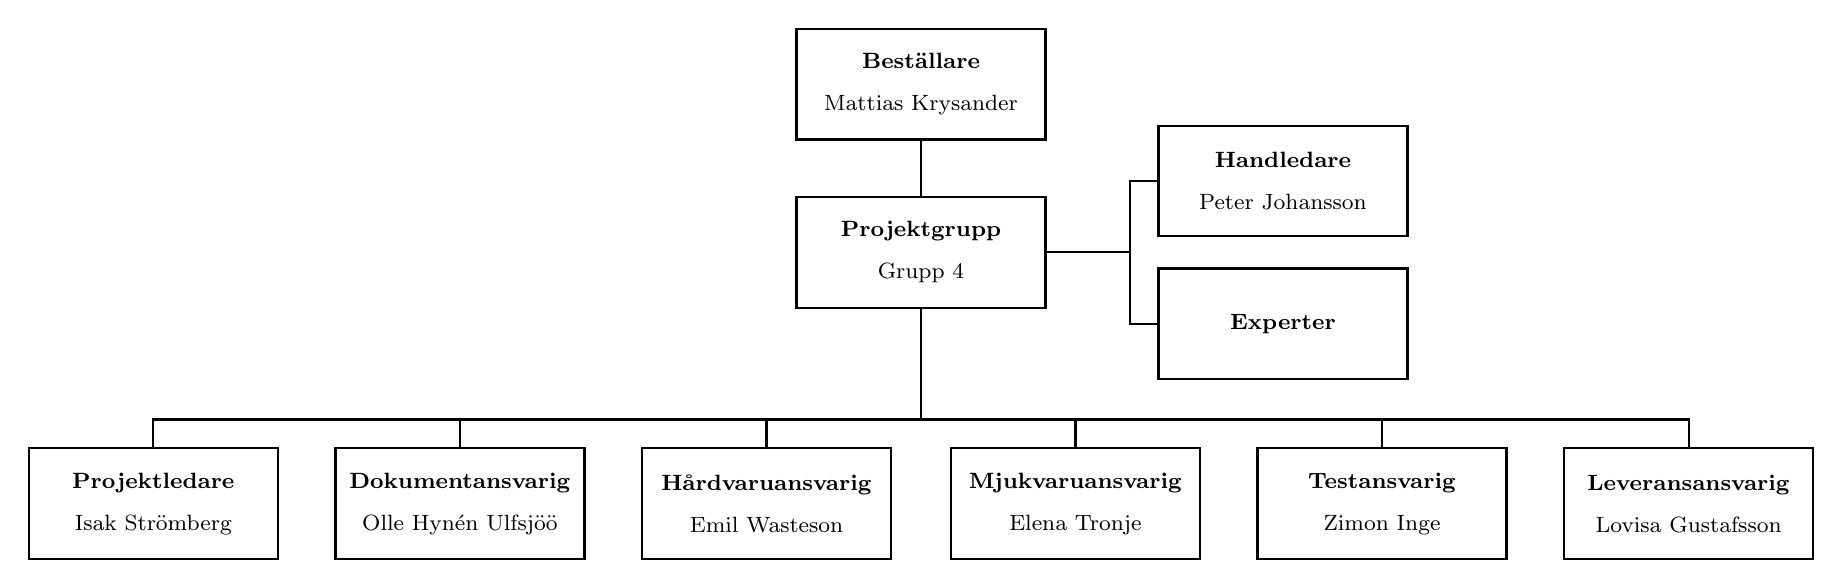
\begin{tikzpicture}
\footnotesize

\tikzset{every node/.style={thick, draw=black, align=center, minimum height=40pt, text width=80pt, minimum width=90pt}}

\node(bestallare) {\textbf{Beställare} \\ \vspace{2mm} Mattias Krysander};

\node[below=20pt] (projektgrupp) at (bestallare.south) {\textbf{Projektgrupp} \\ \vspace{2mm} Grupp 4};

\node[above right=-15pt and 40pt of projektgrupp] (handledare) {\textbf{Handledare} \\ \vspace{2mm} Peter Johansson};
\node[below right=-15pt and 40pt of projektgrupp] (experter) {\textbf{Experter}};

\node[below left = 50pt and -35pt of projektgrupp] (pm3) {\textbf{Hårdvaruansvarig} \\ \vspace{2mm} Emil Wasteson};
\node[below right = 50pt and -35pt of projektgrupp] (pm4) {\textbf{Mjukvaruansvarig} \\ \vspace{2mm} Elena Tronje};
\node[left = 20pt of pm3] (pm2) {\textbf{Dokumentansvarig} \\ \vspace{2mm} Olle Hynén Ulfsjöö};
\node[left = 20pt of pm2] (pm1) {\textbf{Projektledare} \\ \vspace{2mm} Isak Strömberg};
\node[right = 20pt of pm4] (pm5) {\textbf{Testansvarig} \\ \vspace{2mm} Zimon Inge};
\node[right = 20pt of pm5] (pm6) {\textbf{Leveransansvarig} \\ \vspace{2mm} Lovisa Gustafsson};

\coordinate (membertop) at ($(projektgrupp.south)+(0,-40pt)$);
\coordinate(helptop) at ($(projektgrupp.east)+(30pt,0)$);

\draw[thick] (projektgrupp) -- (membertop)
	(pm1.north) |- (membertop) -| (pm6.north)
	(pm2.north) |- (membertop) -| (pm5.north)
	(pm3.north) |- (membertop) -| (pm4.north)
	
	(projektgrupp.east) -- (helptop)
	(handledare.west) -| (helptop) |- (experter.west)
	
	(bestallare.south) -- (projektgrupp.north);
\end{tikzpicture}
\end{document}